\documentclass[11pt,article,oneside]{memoir}
\usepackage{org-preamble-pdflatex}


\usepackage{graphicx}
% We will generate all images so they have a width \maxwidth. This means
% that they will get their normal width if they fit onto the page, but
% are scaled down if they would overflow the margins.
\makeatletter
\def\maxwidth{\ifdim\Gin@nat@width>\linewidth\linewidth
\else\Gin@nat@width\fi}
\makeatother
\let\Oldincludegraphics\includegraphics
\renewcommand{\includegraphics}[1]{\Oldincludegraphics[width=\maxwidth]{#1}}

\title{\bigskip \bigskip Supplementary Material for \emph{Important, Unique, Central: Species'
Relevance in Food Webs} }

%\author{true\\true}

\author{\Large Giulio Valentino Dalla Riva\vspace{0.05in} \newline\normalsize\emph{University of Canterbury, New Zealand} \newline\footnotesize \url{gvd16@uclive.ac.nz}\vspace*{0.2in}\newline  \and \Large Carey E. Priebe\vspace{0.05in} \newline\normalsize\emph{John Hopkins University, MD, USA} \newline\footnotesize \url{}\vspace*{0.2in}\newline }

%\author{Giulio Valentino Dalla Riva (University of Canterbury, New Zealand) \and Carey E. Priebe (John Hopkins University, MD, USA)}

\date{}

\begin{document}  
\setkeys{Gin}{width=1\textwidth} 	
%\setromanfont[Mapping=tex-text,Numbers=OldStyle]{Minion Pro} 
%\setsansfont[Mapping=tex-text]{Minion Pro} 
%\setmonofont[Mapping=tex-text,Scale=0.8]{Pragmata}
\chapterstyle{article-4} 
\pagestyle{kjh}

\published{February 2016.}

\maketitle



\section{Supplementary Methods}\label{supplementary-methods}

\subsection{The Random Dot Product Graph model: context and
details}\label{the-random-dot-product-graph-model-context-and-details}

In our paper we introduce the Random Dot Product Graph model (RDPG) for
food webs. This model can be seen as a special case of the stochastic
block graph model, originally developed for the analysis of undirected
social networks (Holland, Laskey, and Leinhardt 1983) and subsequently
generalised to directed graphs (Wang and Wong 1987). Under the
stochastic blockmodel assumptions, each of the nodes of a network are
assigned to one of \(K\) distinct blocks. The probability of a link
within and between the \(K\) blocks are given by the model parameters.
However, in practice we do not observe the assignment of the nodes to
the blocks; rather, we observe the interactions between nodes and try to
estimate the assignment. This approach has been by some recent models
for food webs (Allesina and Pascual 2009, baskerville2011spatial).
Recently, it has been proved that a consistent block estimator (i.e., an
estimator such that the proportion of nodes assigned to the wrong group
converges in probability to zero as the number of the species grows to
infinity) based on the spectral partitioning of the normalized Laplacian
of the adjacency matrix exist (Rohe, Chatterjee, and Yu 2011). The RDPG
model can be read as a particular case of the stochastic blockmodels
(Fishkind et al. 2013) where each species is assigned to different block
and the probability of the interaction from block (species) \(i\) to
block (species) \(j\) depends on the distance between \(i\) and \(j\) in
the metric space, i.e., it is given by the dot product of the two
position vectors. We observe the realized interactions and estimate the
position of the species in the metric space. Notice that, as the
interaction probabilities are given by the pairwise distances, and the
observed graph is an outcome of a stochastic process defined by those
probabilities, any transformation of the metric space preserving the
distance structure begets an equivalent model.

In particular, the RDPG model we consider in the paper is a
generalization of the RDPG model to binary directed graphs: as the
interactions are no more symmetric, we have to consider a pair of metric
spaces, an \emph{inward} and an \emph{outward} one. We use an estimator
based on the spectral partitioning of adjacency (non Laplacian) matrix
of a graph (Sussman et al. 2012) to estimate species positions in the
underlying metric space.

With some abuse of notation, we let \(A\) denote both a food web and its
adjacency matrix. Let the three matrices \(L, \Sigma, R\) denote a
singular value decomposition of the adjacency matrix \(A\) (a food web
with \(S\) species). Thus, the matrices \(L, \Sigma, R\) satisfy
\(A = L \times \Sigma \times R^t\); \(L\) and \(R\) are real, orthogonal
\(S \times S\) matrices; \(\Sigma\) is an \(S \times S\) diagonal matrix
whose entries are the singular values of \(A\), in a non-decreasing
order. Fixed a model dimension \(d\), we define three new matrices:

\begin{enumerate}
\def\labelenumi{\arabic{enumi}.}
\tightlist
\item
  \(L'\), an \(S \times d\) matrix given by the first \(d\) columns of
  \(L\);
\item
  \(R'\), an \(S \times d\) matrix given by the first \(d\) columns of
  \(R\);
\item
  \(\left(\Sigma'\right)^{1/2}\), an \(d \times d\) diagonal matrix
  defined by the square root of the first \(d\) entries of \(\Sigma\),
  i.e., the square root of the first \(d\) greatest singular values of
  \(A\).
\end{enumerate}

Then, we let \(\hat{L}\) denote the rescaled matrix
\(L' \times \left( \Sigma'\right)^{1/2}\) and we let \(\hat{R}\) denote
the rescaled matrix \(\left( \Sigma'\right)^{1/2} \times R'\). The two
matrices \(\hat{l}\) and \(\hat{R}\) capture the \(d\) leading traits
for the community of species as prey and predators: the rows of
\(\hat{L}\) define the species' vulnerability functional traits
(\emph{outward}) and the rows of \(\hat{R}\) define the foraging
functional traits (\emph{inward}) of the species in \(A\). We call the
column binding of \(\hat{L}\) and \(\hat{R}\) the species functional
traits as both prey and predators (\emph{total}).

Notice that although \(\hat{L}\) and \(\hat{R}\) are not uniquely
defined, as any orthogonal transformation of those matrices preserve
their dot product (and hence the distance between the estimated
stochastic food web's backbone and its observed adjacency matrix), the
species' relative position and the induced pairwise distance structure
in the abstract functional space are uniquely defined. The measures we
introduce in the paper are based on the invariant structure of the food
web, rather then on the absolute position of the species.

Different approaches are available for the choice of a suitable
dimension \(d\) range. This akin to a dimensionality reduction problem,
discussed for the Principal Component Analysis scenario in (Jolliffe
2002). The available methods include \emph{a priori} selection
procedures (e.g., the visual analysis of the singular values scree plot
(Cattell 1966), hard singular values thresholding (Chatterjee and others
2014,Gavish and Donoho (2014)) or the maximization of a profile
likelihood function (Zhu and Ghodsi 2006)) and \emph{a posteriori}
maximization of a goodness-of-fit criterion, as we exampled in (Dalla
Riva and Stouffer 2015). In the datasets analysed all the previous
methods provided compatible results.

\subsubsection{The RDPG based measures}\label{the-rdpg-based-measures}

Let \(X(A)\) denote the matrix of (outward, inward or total) functional
traits of the species in the food web \(A\). As we saw above, the
pairwise distance structure induced by \(X(A)\) is uniquely defined, and
hence it is possible to investigate the distribution of the species in
the functional traits space just estimated. In particular, we define the
(outward, inward or total) \emph{uniqueness} of a species \(i\) in the
food web \(A\) as the mean distance between \(i\) and every other
species \(j\) in the (outward, inward or total) functional traits space.
Let \(d\left(p,q\right)\) denote the \(d\) dimensional euclidean
distance between the point \(p\) and \(q\); let
\(\langle f(i,j) \rangle_j\) be the mean of the function \(f\) over all
the species \(j\) except \(i\). That is,
\(\langle f(i,j) \rangle_j = \frac{1}{S}\sum_{j \neq i}(f(i,j))\). Then,
the \textbf{uniqueness} of species \(i\) is defined as:

\begin{equation}
\mbox{uniqueness($i$)} := \langle d\left( X(A)_i,X(A)_j\right)\rangle_j
\end{equation}

Let \(M\) denote a \(N \times M\) matrix: we denote \(M^{d(i)}\) the
matrix obtained by dropping the \(i\)-th column and row from \(M\); te
denote \(M^{r(i)}\) the matrix obtained by removing just the \(i\)-th
row from \(M\). Let \(W\) denote another \(N \times M\) matrix. We
define \(M_{proc}(W)\) as the Procrustes transformation (i.e., a
combination of translation, rotation and uniform rescaling) of \(M\) of
minimal distance to \(W\); we will drop the argument \((W)\) from the
notation whenever it is clear from the context. Finally, we denote
\(||M||_F\) the squared sum of entries of \(M\), i.e., the Frobenius
norm of the matrix \(M\) . In particular, \(||M_{proc}(W) - W||_F\) is
also called the Procrustes distance between \(M\) and \(W\) (Dryden and
Mardia 1998).

We compute the matrix
\[\bigg[X\left(A^{d(i)}\right)\bigg]_{proc}\bigg(X\left(A\right)^{r(i)}\bigg) \, ,\]
that is, the Procrustes transformation of \(X\left(A^{d(i)}\right)\) of
minimal distance to \(X(A)^{r(i)}\) and we denote it
\(\hat{X}\left(A^{d(i)}\right)\). We define the rank \(d\)
\textbf{strain} of the species \(i\) as the sum of squared entries of
the differences between \(X(A)^{r(i)}\) and
\(\hat{X}\left(A^{d(i)}\right)\). Being \(X(A)\) the matrix of either
the inward, outward or total \(d\) dimensional functional traits, we
will speak of species' \emph{inward}, \emph{outward} or \emph{total}
strain, respectively. In formula:

\begin{equation}
\mbox{strain($i$)} := ||X(A)^{r(i)} - \hat{X}\left(A^{d(i)}\right)||_F
\end{equation}

Computing the strain of species \(i\) reduces to computing the ordinary
Procrustes distance between the matrices \(X(A)^{r(i)}\) and
\(X\left(A^{d(i)}\right)\), which is implemented by the \emph{procOPA}
function in the R package \emph{shapes} (Dryden 2013,R Core Team
(2014)).

Finally, we identify the (outward, inward, total) diversity of the food
web \(A\) as the volume of the convex hull containing all the species in
the (outward, inward, total) functional traits space. Conceptually
borrowing from the functional traits literature, we define the
\textbf{contribution} of the species \(i\) to the food web (outward,
inward, total) \textbf{functional diversity} as the volume difference of
the convex hulls of \(X\left(A\right)\) and \(X\left(A\right)^{r(i)}\).
We compute the convex hulls and their volumes using Qhull (Barber,
Dobkin, and Huhdanpaa 1996), through the \emph{R} package
\emph{geometry} (Habel et al. 2014).

\subsubsection{Keystone Centralities}\label{keystone-centralities}

We compare our novel measures with six graph centralities measures that
have been adopted to idenfity keystone species in ecological networks.
In particular, for each species \(i\) in the food web, we consider:

\begin{itemize}
\tightlist
\item
  the betweennessi (BC, Freeman 1977) of species \(i\), given by the
  number \(s_{jij'}\) of shortest paths connecting every pair \(j,j'\)
  of species in the food web traversing species \(i\)i, weighted by the
  total number \(s_{jj'}\) of paths between \(j\) and \(j'\):
  \[BC(i) := \frac{s_{jij'}}{s_{jj'}}\]
\item
  the closeness (CC, Bavelas 1950) of species \(i\), defined as the
  reciprocal of the sum of the path distances, \(d_p(\cdot)\), from
  \(i\) to every other species \(j\) in the food web:
  \[CC(i) := \left( \sum_{j \neq i} d_p(j,i)\right)^{-1}\]
\item
  the degree (DC) of species \(i\), measuring the number of interactions
  involving the species \(i\) (both as a predator or as a prey):
  \[DC(i) := |\left\{j \in A | i \to j \mbox{ or } j \to i \right\}|\]
\item
  the eigenvector centrality (EC, Bonacich 1987) of species \(i\), that
  is a graph centrality satisfying the request that the score of each
  species \(i\) in the food web is proportional to the sum of the
  centrality scores of the species interacting with \(i\). The values of
  EC are computed as the entries of the first eigenvector of \(A\).
\item
  the information centrality (IC, Stephenson and Zelen 1989) of species
  \(i\), that is the harmonic mean of the resistance distances (Klein
  and Randić 1993) toward the species \(i\). Let \(I_{ji}\) denote the
  resistance distance from \(j\) to \(i\), then:
  \[IC(i) := \frac{S}{\sum_{j \neq i}\left(I_{ji}\right)^{-1}}\]
\item
  the subgraph centrality (SC, Estrada and Rodriguez-Velazquez 2005) of
  species \(i\), which counts the number of returning loops starting
  from species \(i\), discounted exponentially by their size. It is
  possible to give a closed expression for IC in terms of the
  exponential of the adjacency matrix \(A\):
  \[SC(i) := \left[ e^A \right]_{ii}\]
\end{itemize}

The above centralities can be computed directly from the adjacency
matrix of the considered food web and are implemented in the \emph{R}
package \emph{igraph} (Csardi and Nepusz 2006). For a discussion of the
interpretation of the previous graph centralities in an ecological
network context, see (Jordán 2009,Jordán, Liu, and Mike (2009)).

\newpage

\section{Data}\label{data}

We analysed five different food webs. We present them graphically using
the \(x\) axis to show the species' omnivory index (adding some noise to
avoid nodes overlap), the \(y\) axis to show the species trophic level,
the size of the nodes to shows species total degree and the color of the
nodes their ranking based on the total strain (deep blue for lower
values, light yellow for higher values).

The original images and the interaction data are available online at the
webpage of the paper.

\newpage

\subsection{Caribbean Sea food web}\label{caribbean-sea-food-web}

We analyse the Caribbean sea food web as compiled by (Opitz 1996). To
observe how our model responds to leveld of taxonomic definitions, we
consider both the original food web, where taxa are defined to the level
of species, and a coarser version where we cluster species into
families.

\begin{figure}[htbp]
\centering
\includegraphics{Images/Webs/Caribbean_Species.pdf}
\caption{Caribbean Sea food web: (above) nodes represent families,
(below) nodes represent species}
\end{figure}

\newpage

\subsection{Serengeti (Baskerville) food
web}\label{serengeti-baskerville-food-web}

\begin{figure}[htbp]
\centering
\includegraphics{Images/Webs/Serengeti_Baskerville.pdf}
\caption{Serengeti National Park food web (by Baskerville)}
\end{figure}

The Serengeti National Park food web was compiled by (Baskerville et al.
2011), notice the increased definition of the plant guilds with respect
to (Visser, Freymann, and Olff 2011). The higher degree of omnivory in
this web is only apparent and is due to the normalisation effect.

\newpage

\subsection{Serengeti (de Visser) food
web}\label{serengeti-de-visser-food-web}

\begin{figure}[htbp]
\centering
\includegraphics{Images/Webs/Serengeti_deVisser.pdf}
\caption{Serengeti National Park food web (de Visser)}
\end{figure}

The Serengeti National Park food web by (Visser, Freymann, and Olff
2011)

\newpage

\subsection{Weddell Sea food web}\label{weddell-sea-food-web}

\begin{figure}[htbp]
\centering
\includegraphics{Images/Webs/Weddell.pdf}
\caption{Weddell Sea food web}
\end{figure}

The Weddell Sea food web is a large marine food web compiled by
(Jennings et al. 2002)

\newpage

\section{Results}\label{results}

\subsection{Weighted networks}\label{weighted-networks}

In the manuscript we presented species strain from binary food webs'
data only. In fact, obtaining estimates for the amount of energy flowing
between a pair of species is often difficult. Therefore, we usually have
a more reliable knowledge of the topological structure of an interaction
network rather than of its weighted version. However, the components of
the species' diets are not equally important. Thus, if the species'
ranking we estimated from the topological data were extremely sensitive
to the interactions' weight its applicability would be limited. On the
other hand, if the topological species' ranking were not affected at all
by the specification of interactions weights, that would rise doubt
about its ecological meaning.

To test the extent to which our \emph{strain} and \emph{mean distance}
measures are robust to the specification of interactions' weights, we
compared the ranking of the species based on topological data with the
rankings we obtained by simulating interactions weights. To do so, we
sampled the interactions weights from a Log-Normal distribution,
truncated so that their minimum value was \(10^{-6}\) and normalised so
that the maximum value was \(1\).

The results we obtained show that the correlation between the
topological and the weighted rankings were significant and positive for
more than \(95\%\) of the simulations. However, the amount of variation
in the weighted ranking explained by the topological ranking had a large
variance (i.e., it spanned the range from almost null to almost one).
Yet, the set of species with higher \emph{strain} and the set of species
with higher \emph{mean distance} as estimated from the topological data
was consistent across the simulated weighted networks, indicating that
our measures are able to identigy the species with distinctively high
ecological importance. Here we just show part of the results (restricted
to the total functional trait space and the the Baskerville's Serengeti
and the Weddell sea food webs), to support the notion that the four
species with highest strain and uniqueness as computed from the binary
webs are consistently in the set of four species with highest strain and
uniqueness as computed from weighted webs.

\newpage

\includegraphics{Images/strain_weight/Serengeti_Baskerville_total.pdf}
\includegraphics{Images/strain_weight/Weddell_total.pdf}

Frequency of presence in the set of four species with the highest strain
as estimated by the simulated weighted networks for the four species
with the highest strain as estimated by the topological networks.

\newpage

\includegraphics{Images/meand_weight/Serengeti_Baskerville_total.pdf}
\includegraphics{Images/meand_weight/Weddell_total.pdf}

Frequency of presence in the set of four species with the highest mean
distance as estimated by the simulated weighted networks for the four
species with the highest mean distance as estimated by the topological
networks.

\newpage

We present here additional results similar to the ones presented in the
main paper. All the original graphic files, the source code used to
produce them, and the data on which they are based are available online
at http://gvdr.github.io.

\newpage

\subsection{Strain}\label{strain}

\begin{figure}[htbp]
\centering
\includegraphics{Images/strains_log.pdf}
\caption{Total strain (log transformed) as function of the model
dimension (rank).}
\end{figure}

We computed the (inward, outward and total) species strain for all the
species in the five food webs.

\newpage

\subsection{Strain distribution}\label{strain-distribution}

We show here the distribution of the 3-dimensional total, inward and
outward strain for the five foodwebs.

\begin{figure}[htbp]
\centering
\includegraphics{Images/Distrs/Caribbean_Speciesdistr.pdf}
\caption{Caribbean Sea food web, nodes represent species}
\end{figure}

\begin{figure}[htbp]
\centering
\includegraphics{Images/Distrs/Caribbean_Familiesdistr.pdf}
\caption{Caribbean Sea food web, nodes represent families}
\end{figure}

\begin{figure}[htbp]
\centering
\includegraphics{Images/Distrs/Serengeti_Baskervilledistr.pdf}
\caption{Serengeti National Park food web (Baskerville)}
\end{figure}

\begin{figure}[htbp]
\centering
\includegraphics{Images/Distrs/Serengeti_deVisserdistr.pdf}
\caption{Serengeti National Park food web (de Visser)}
\end{figure}

\begin{figure}[htbp]
\centering
\includegraphics{Images/Distrs/Weddelldistr.pdf}
\caption{Weddell Sea food web}
\end{figure}

\newpage

\subsection{Strain correlation}\label{strain-correlation}

\begin{figure}[htbp]
\centering
\includegraphics{Images/Strains_corr.pdf}
\caption{Correlation of the species' total strain as a function of the
model dimension}
\end{figure}

The choice of the model dimension does not substantially affect the
ranking of species' strain, supporting the notion that the measure is
robust to model parameters. Deep blue for lower coefficients of
determination, light yellow for higher values. All correlations are
significant.

\newpage

\subsection{Uniqueness correlation}\label{uniqueness-correlation}

\begin{figure}[htbp]
\centering
\includegraphics{Images/Md_corr.pdf}
\caption{Correlation of the species' total uniqueness as a function of
the model dimension}
\end{figure}

The choice of the model dimension does not substantially affect the
ranking of species' uniqueness, supporting the notion that the measure
is robust to model parameters. The rows show inward uniqueness, outward
uniqueness and total uniqueness respectively. Deep blue for lower
coefficients of determination, light yellow for higher values. Blank
cells represent non significant correlations.

\newpage

\subsection{Strain vs.~Uniqueness}\label{strain-vs.uniqueness}

\begin{figure}[htbp]
\centering
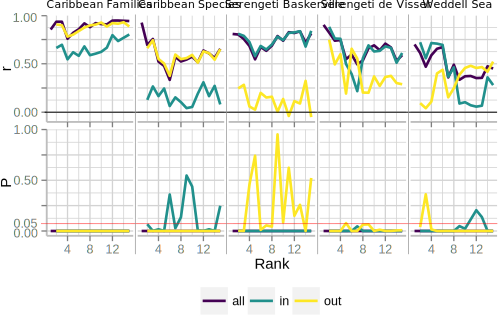
\includegraphics{Images/indir.pdf}
\caption{Correlation between species' strain and uniqueness}
\end{figure}

There's a significant correlation between species' strain (inward,
outward or total) and uniqueness (inward, outward or total). The
correlation does not grow with the model dimension (and for the
Caribbean Sea food web (species level), the Serengeti de Visser food web
and the Weddell Sea food web it decreases).

\newpage

\subsection{Strain vs.~Keystone
centralities}\label{strain-vs.keystone-centralities}

\begin{figure}[htbp]
\centering
\includegraphics{Images/Strain_corr_rP.pdf}
\caption{Correlation between species' strain and six classic centrality
measures}
\end{figure}

There's a significant correlation between species' strain (inward,
outward or total) and the six centrality measures we considered. We
observe more often significant correlations at the lower model
dimensions and the coefficients of determination do not grow with model
dimensions. This suggest the conclusion the the food web are inherently
low dimensional.

\newpage

\subsection{Uniqueness vs.~Keystone
centralities}\label{uniqueness-vs.keystone-centralities}

\begin{figure}[htbp]
\centering
\includegraphics{Images/MeanD_Keystones.png}
\caption{Correlation between species' uniqueness and six classic
centrality measures}
\end{figure}

As for the species' strain, there's a significant correlation between
species' uniqueness (inward, outward or total) and the six centrality
measures we considered. We observe more often significant correlations
at the lower model dimensions and the coefficients of determination do
not grow with model dimensions.

\newpage

\hyperdef{}{references}{\label{references}}
\section*{Bibliography}\label{bibliography}
\addcontentsline{toc}{section}{Bibliography}

\hyperdef{}{ref-allesina2009food}{\label{ref-allesina2009food}}
Allesina, Stefano, and Mercedes Pascual. 2009. ``Food web models: A plea
for groups.'' \emph{Ecology letters} 12(7): 652--662.

\hyperdef{}{ref-barber1996quickhull}{\label{ref-barber1996quickhull}}
Barber, C Bradford, David P Dobkin, and Hannu Huhdanpaa. 1996. ``The
quickhull algorithm for convex hulls.'' \emph{ACM Transactions on
Mathematical Software (TOMS)} 22(4): 469--483.

\hyperdef{}{ref-baskerville}{\label{ref-baskerville}}
Baskerville, Edward B et al. 2011. ``Spatial guilds in the serengeti
food web revealed by a bayesian group model.'' \emph{PLoS Computational
Biology} Vol. 7(No. 12): e1002321.

\hyperdef{}{ref-bavelas1950communication}{\label{ref-bavelas1950communication}}
Bavelas, Alex. 1950. ``Communication patterns in task-oriented groups.''
\emph{Journal of the acoustical society of America} 22(6).

\hyperdef{}{ref-bonacich1987power}{\label{ref-bonacich1987power}}
Bonacich, Phillip. 1987. ``Power and centrality: A family of measures.''
\emph{American journal of sociology}: 1170--1182.

\hyperdef{}{ref-cattell1966scree}{\label{ref-cattell1966scree}}
Cattell, Raymond B. 1966. ``The scree test for the number of factors.''
\emph{Multivariate behavioral research} 1(2): 245--276.

\hyperdef{}{ref-chatterjee2014matrix}{\label{ref-chatterjee2014matrix}}
Chatterjee, Sourav, and others. 2014. ``Matrix estimation by universal
singular value thresholding.'' \emph{The Annals of Statistics} 43(1):
177--214.

\hyperdef{}{ref-igraph}{\label{ref-igraph}}
Csardi, Gabor, and Tamas Nepusz. 2006. ``The igraph software package for
complex network research.'' \emph{InterJournal} Complex Systems: 1695.
\url{http://igraph.org}.

\hyperdef{}{ref-dallariva2015exploring}{\label{ref-dallariva2015exploring}}
Dalla Riva, Giulio V., and Daniel B. Stouffer. 2015. ``Exploring the
evolutionary signature of food webs' backbones using functional
traits.'' \emph{Oikos} Online early view(10.1111/oik.02305).

\hyperdef{}{ref-dryden1998statistical}{\label{ref-dryden1998statistical}}
Dryden, Ian L, and Kanti V Mardia. 1998. 4 \emph{Statistical shape
analysis}. Wiley Chichester.

\hyperdef{}{ref-shapes}{\label{ref-shapes}}
Dryden, Ian L. 2013. \emph{Shapes: Statistical shape analysis}.
\url{http://CRAN.R-project.org/package=shapes}.

\hyperdef{}{ref-estrada2005subgraph}{\label{ref-estrada2005subgraph}}
Estrada, Ernesto, and Juan A Rodriguez-Velazquez. 2005. ``Subgraph
centrality in complex networks.'' \emph{Physical Review E} Vol. 71(No.
5): 056103.

\hyperdef{}{ref-fishkind2013consistent}{\label{ref-fishkind2013consistent}}
Fishkind, Donniell E et al. 2013. ``Consistent adjacency-spectral
partitioning for the stochastic block model when the model parameters
are unknown.'' \emph{SIAM Journal on Matrix Analysis and Applications}
34(1): 23--39.

\hyperdef{}{ref-freeman1977set}{\label{ref-freeman1977set}}
Freeman, Linton C. 1977. ``A set of measures of centrality based on
betweenness.'' \emph{Sociometry} 40(1): 35--41.

\hyperdef{}{ref-gavish2014optimal}{\label{ref-gavish2014optimal}}
Gavish, Matan, and David L Donoho. 2014. ``The optimal hard threshold
for singular values is.'' \emph{Information Theory, IEEE Transactions
on} 60(8): 5040--5053.

\hyperdef{}{ref-geometry}{\label{ref-geometry}}
Habel, Kai et al. 2014. \emph{Geometry: Mesh generation and surface
tesselation}. \url{http://CRAN.R-project.org/package=geometry}.

\hyperdef{}{ref-holland1983stochastic}{\label{ref-holland1983stochastic}}
Holland, Paul W, Kathryn Blackmond Laskey, and Samuel Leinhardt. 1983.
``Stochastic blockmodels: First steps.'' \emph{Social networks} 5(2):
109--137.

\hyperdef{}{ref-Weddell}{\label{ref-Weddell}}
Jennings, S et al. 2002. ``Long-term trends in the trophic structure of
the north sea fish community: Evidence from stable-isotope analysis,
size-spectra and community metrics.'' \emph{Marine Biology} Vol. 141(No.
6): 1085--1097.

\hyperdef{}{ref-jolliffe2002principal}{\label{ref-jolliffe2002principal}}
Jolliffe, Ian T. 2002. \emph{Principal component analysis}.
Springer-Verlag.

\hyperdef{}{ref-jordan2009keystone}{\label{ref-jordan2009keystone}}
Jordán, Ferenc. 2009. ``Keystone species and food webs.''
\emph{Philosophical Transactions of the Royal Society B: Biological
Sciences} Vol. 364(No. 1524): 1733--1741.

\hyperdef{}{ref-jordan2009trophic}{\label{ref-jordan2009trophic}}
Jordán, Ferenc, Wei-Chung Liu, and Ágnes Mike. 2009. ``Trophic field
overlap: A new approach to quantify keystone species.'' \emph{Ecological
Modelling} Vol. 220(No. 21): 2899--2907.

\hyperdef{}{ref-klein1993resistance}{\label{ref-klein1993resistance}}
Klein, Douglas J, and M Randić. 1993. ``Resistance distance.''
\emph{Journal of Mathematical Chemistry} 12(1): 81--95.

\hyperdef{}{ref-caribbean}{\label{ref-caribbean}}
Opitz, S. 1996. ``Trophic interactions in caribbean coral reefs.''
\emph{The WorldFish Center Working Papers}.

\hyperdef{}{ref-R}{\label{ref-R}}
R Core Team. 2014. \emph{R: A language and environment for statistical
computing}. Vienna, Austria: R Foundation for Statistical Computing.
\url{http://www.R-project.org/}.

\hyperdef{}{ref-rohe2011spectral}{\label{ref-rohe2011spectral}}
Rohe, Karl, Sourav Chatterjee, and Bin Yu. 2011. ``Spectral clustering
and the high-dimensional stochastic blockmodel.'' \emph{The Annals of
Statistics}: 1878--1915.

\hyperdef{}{ref-stephenson1989rethinking}{\label{ref-stephenson1989rethinking}}
Stephenson, Karen, and Marvin Zelen. 1989. ``Rethinking centrality:
Methods and examples.'' \emph{Social Networks} Vol. 11(No. 1): 1--37.

\hyperdef{}{ref-sussman2012consistent}{\label{ref-sussman2012consistent}}
Sussman, Daniel L et al. 2012. ``A consistent adjacency spectral
embedding for stochastic blockmodel graphs.'' \emph{Journal of the
American Statistical Association} 107(499): 1119--1128.

\hyperdef{}{ref-deVisser}{\label{ref-deVisser}}
Visser, Sara N de, Bernd P Freymann, and Han Olff. 2011. ``The serengeti
food web: Empirical quantification and analysis of topological changes
under increasing human impact.'' \emph{Journal of Animal Ecology} Vol.
80(No. 2): 484--494.

\hyperdef{}{ref-wang1987stochastic}{\label{ref-wang1987stochastic}}
Wang, Yuchung J, and George Y Wong. 1987. ``Stochastic blockmodels for
directed graphs.'' \emph{Journal of the American Statistical
Association} 82(397): 8--19.

\hyperdef{}{ref-zhu2006automatic}{\label{ref-zhu2006automatic}}
Zhu, Mu, and Ali Ghodsi. 2006. ``Automatic dimensionality selection from
the scree plot via the use of profile likelihood.'' \emph{Computational
Statistics \& Data Analysis} Vol. 51(2): 918--930.

\end{document}
